\documentclass[tikz,border=2pt]{standalone}
\usepackage{amsmath,amssymb}
\usepackage{tikz}

\begin{document}
% The complement A^c is everything in S outside A, so its probability is 1 - P(A).
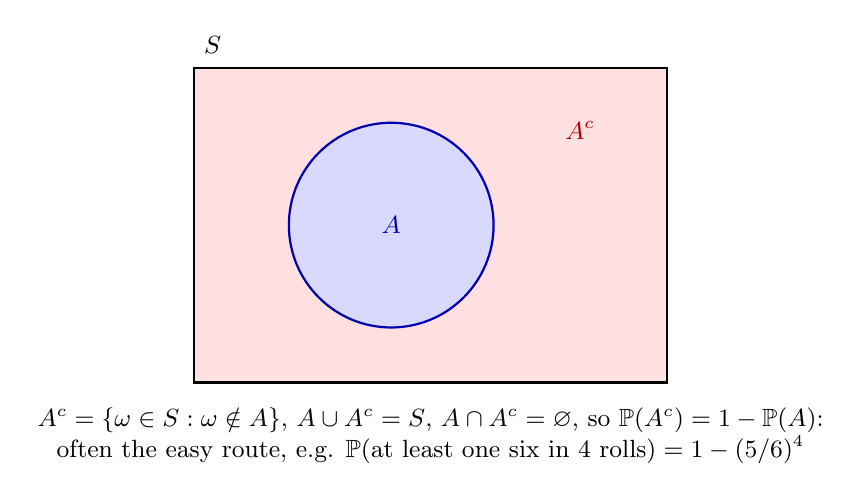
\begin{tikzpicture}[every node/.style={font=\small}]
	\fill[red!12] (-3,-2) rectangle (3,2);
	\fill[white] (-0.5,0) circle (1.3);
	\fill[blue!15] (-0.5,0) circle (1.3);
	\draw[thick] (-3,-2) rectangle (3,2);
	\draw[thick, blue!70!black] (-0.5,0) circle (1.3);
	\node[blue!70!black] at (-0.5,0) {$A$};
	\node[red!70!black] at (1.9,1.2) {$A^{c}$};
	\node[anchor=south west] at (-3,2.05) {$S$};
	\node[anchor=north, align=flush center, text width=10cm] at (0,-2.2) {$A^{c}=\{\omega\in S:\omega\notin A\}$, $A\cup A^{c}=S$, $A\cap A^{c}=\varnothing$, so $\mathbb{P}(A^{c})=1-\mathbb{P}(A)$: often the easy route, e.g. $\mathbb{P}(\text{at least one six in 4 rolls})=1-(5/6)^4$};
\end{tikzpicture}
\end{document}
